\documentclass[11pt]{article}
\usepackage{lmodern,setspace,amsmath,amssymb,amsfonts,amsthm,graphicx,multicol,grffile,float}
\usepackage{mathtools}
\usepackage{authblk,url,csvsimple,cuted,dblfloatfix,parskip}
\usepackage[a4paper, top=0.9in, bottom=1.05in, left=1.01in, right=1.01in]{geometry}
\usepackage[polish]{babel}
\usepackage[utf8]{inputenc}
\usepackage[unicode]{hyperref}
\usepackage{listings}
\usepackage{booktabs}

\usepackage[linesnumbered,ruled,vlined]{algorithm2e}
\DontPrintSemicolon
\SetKw{Break}{break}
\SetKw{Continue}{continue}
\DeclareMathOperator*{\argmax}{arg\!max}

\title{PTSZ - Zadanie 1 - Problem $1|r_i|\Sigma w_i U_i$}
\author{Dariusz Max Adamski 136674 (grupa I9, godzina 8:00)}
\affil{dariusz.adamski@student.put.poznan.pl}
\date{Data oddania: \today}

\def\code#1{\texttt{#1}}

\begin{document}

\maketitle

\section*{Wstęp}

W tym sprawozdaniu opisane jest podejście rozwiązujące problem szeregowania zadań na jednej maszynie, z czasami startowymi i minimalizacją ważonej liczby zadań spóźnionych.

\section{Generator instancji}

\begin{algorithm}
\caption{Algorytm generatora instancji dla problemu $1|r_i|\Sigma w_i U_i$}
$\mu_p = 5; \mu_s = 7; \sigma_w = 2$ \;
$t = \mu_p$ \;
\For{i \in 1 \dots n}{
    $r_i \coloneqq \max \{ 0, \lfloor \text{Normal}(t, \mu_p) \rfloor \}$ \;
    $p_i \coloneqq 1 + \text{NegativeBinomial}(\mu_p, 2) $ \;
    $d_i \coloneqq r_i + p_i + \text{NegativeBinomial}(\mu_s, 2) $ \;
    $w_i \coloneqq \max \{ 1, \lfloor \text{Normal}(p(\frac{p}{d-r} + 0.5), \sigma_w) \rfloor \} $ \;
    \If{$\text{Bernoulli}(step) = 1$}{
        $\text{step} \coloneqq \max\{0.05, \text{Beta}(2, 10)\} $ \;
        $t \coloneqq t + \text{Binomial}(\mu_p + \mu_s, 0.5) $ \;
    }
}
Potasuj losowo zadania
\end{algorithm}

\begin{figure}[b]
\caption{Wizualizacje wygenerowanych instancji o wielkości 100, 200 i 400}
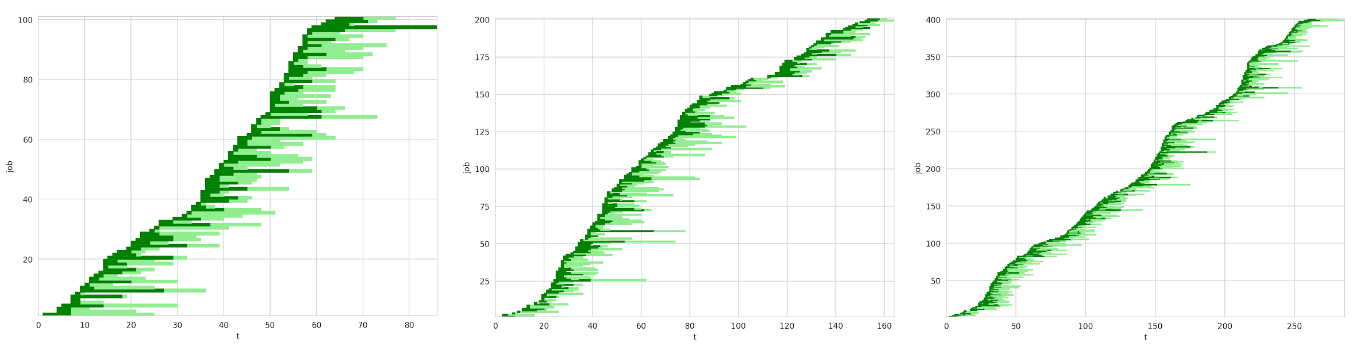
\includegraphics[width=\textwidth]{inst.png}
\centering
\end{figure}

\subsection{Opis algorytmu}

\begin{figure}[t]
\caption{Rozkłady prawdopodobieństwa użyte w algorytmie generatora}
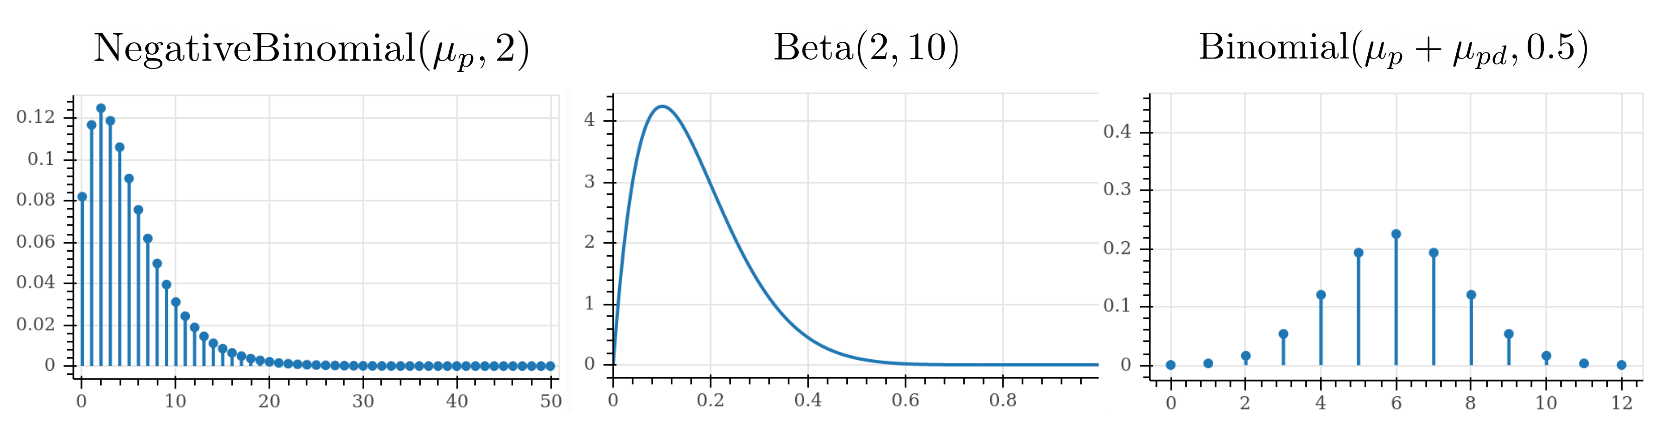
\includegraphics[width=\textwidth]{dist.png}
\centering
\end{figure}

Dla każdego zadania czas gotowości $r_i$ jest losowany z rozkładu normalnego wyśrodkowanego na aktualnym czasie symulacji, z odchyleniem standardowym równym średniemu czasowi przetwarzania $\mu_p$, przy czym czas gotowości nie może być mniejszy od 0, a wartość jest zaokrąglana funkcją podłoga. W efekcie, nawet jeśli symulacja jest w czasie $t$, to czas gotowości może przypaść na wcześniejszy moment, przez co zadanie może kolidować z innym wcześniejszym. 

Czas przetwarzania $p_i$ jest losowany z dyskretnego rozkładu Pascala ze średnią wartością $\mu_p$ i eksperymantalnie dobranym parametrem $\varphi$, równym 2. Do tej wartości dodawane jest jeszcze 1, żeby minimalną wartością czasu przetwarzania było 1, a nie 0. Podobnie losowany jest oczekiwany czas zakończenia $d_i$, przy czym minimalną wartością jest $r_i + p_i$, a do tego jest dodawany luz, który jest losowany z rozkładu Pascala ze średnią wartością $\mu_s$ i $\varphi$ równym 2. Pierwszy z rozkładów jest zwizualizowany na rysunku 2. Wynika z niego, że po dodaniu 1, najczęstszym czasem przetwarzania jest 3, często są też zadania o długości 1 i 2. Większość zadań ma czas przetwarzania mniejszy od 10, ale mogą zdarzyć się nawet zadania o długości 20 lub nawet większej, chociaż prawdopodobieństwo tego jest niskie.

Waga zadania $w_i$ jest losowana z rozkładu normalnego o średniej $p(0.5 + p/(d - r))$ z odchyleniem standardowym $\sigma_w$. Chciałem, żeby waga była proporcjonalna do czasu przetwarzania, ale żeby zadania, których nie można ,,przesuwać'' (te dla których $p/(d - r)$ jest bliżej 1) miały większą wagę (odwrotnie proporcjonalnie do luzów).

Ciekawą według mnie częścią algorytmu jest to, że czas symulacji nie jest zwiększany jednolicie, ale z pewnym prawdopodobieństwem $step$. Po każdym zadaniu, jeśli wartość próby Bernoulliego wyniesie 1, to czas symulacji jest zwiększany o krok losowany z rozkładu dwumianowego, ze średnią wartością wartością równą $\mu_p + \mu_s$ (trzeci wykres na rysunku 1). Następnie ponownie losowane jest prawdopodobieństwo zwiększenia czasu symulacji z rozkładu Beta o parametrach 2 i 10, przy czym minimalne prawdopodobieństwo ma wynośić 5\%. Rozkład Beta został dobrany eksperymentalnie tak, żeby większość prawdopodobieństw była mniejsza od 0.3, ale żeby czasami mogły być też większe. Takie zachowanie skutkuje wygięciami instancji (widocznymi na rysunku 1), które mają symulować momenty, w których na maszynę nie wpływa wiele nowych zadań.

\section{Algorytm szeregowania}

\begin{algorithm}
\caption{Algorytm dla problemu $1|r_i|\Sigma w_i U_i$}
\While{T \neq \varnothing}{
$\var{assigned} \coloneqq 0$ \;
$t \coloneqq 0$ \;
\While{t < $\max d$}{
$T_{\text{valid}} \coloneqq \{ T_j \in T \mid d_j - t \geq p_j \land \lnot \var{scheduled}(\max \{t, r_j\}, p_j) \}$ \;
\If{$T_{\text{valid}} = \varnothing$}{
    $t \coloneqq \max \{t + 1, \min_{T_j \in T} r_j \}$ \;
    \Continue \;
}
$T_{\text{best}} \coloneqq T_{\text{valid}} \left[ \argmax_{T_j \in T_{\text{valid}}} \frac{w_j}{d_j - t} \right] $ \;
$t_1 \coloneqq \max \{ t, r_{\text{best}} \} $ \;
$t_2 \coloneqq t_1 + p_{\text{best}}$ \;
Zaplanuj zadanie $T_{\text{best}}$ w czasie $t_1 \dots t_2$ \;
$T \coloneqq T \setminus \{ T_{\text{best}} \}$ \;
$t \coloneqq t_2$ \;
$\var{assigned} \coloneqq \var{assigned} + 1$ \;
}
\If{$\text{assigned} = 0$}{\Break}
}
Zaplanuj pozostałe zadania z $T$ w dowolnej kolejności
\end{algorithm}

\subsection{Oznaczenia}

Zbiór $T$ początkowo zawiera wszystkie zadania $T_1 \dots T_n$. Gdy zadanie jest dodane do uszeregowania, usuwane jest z tego zbioru.

Zmienna $assigned$ zawiera liczbę zaplanowanych zadań w danej iteracji. Jeśli pod koniec iteracji ta zmienna jest równa zero, to z algorytmu wynika, że nie można już zaplanować więcej zadań, tak żeby wykonały się przed ,,due date''.

Zmienna $t$ oznacza aktualny czas symulacji.

Zbiór $T_{\text{valid}}$ zawiera zadania $T_j$, które mogą być przypisane w chwili $t$, lub późniejszej, tak aby zakończyły się przed due date $d_j$ i nie kolidowały z innymi zaplanowanymi zadaniami.

Predykat $\text{scheduled}(t, p)$ przyjmuje wartość prawdziwą, jeśli jest już zaplanowane jakieś zadanie w przedziale $t \dots t + p$ (lub jego podzbiorze). W przeciwnym wypadku predykat przyjmuje wartość fałszywą.

\subsection{Opis algorytmu}

Działanie algorytmu szeregowania jest bardzo proste. Dla danego punktu w czasie, według heurystyki wybierane jest ,,najlepsze'' zadanie, które nie koliduje z innymi już zaplanowanymi zadaniami i może się zakończyć przed due date $d_i$. Jeśli $t < r_i$, to czas jest ustawiany na $r_i$, a następnie robiony jest krok czasowy równy czasowi wykonania tego zadania $p_i$. Gdy czas symulacji jest równy lub większy od największego due date, algorytm jest powtarzany, żeby zapełnić wolne miejsca w uszeregowaniu, które powstały w wyniku planowania zadań z czasem gotowości $r_i$ większym od aktualnego czasu symulacji $t$.

Według wybranej heurystyki najlepsze zadanie ma największą wartość wyrażenia $w_i/(d_i - t)$, co oznacza, że w pierwszej kolejności wybierane są zadania z największą wagą i najkrótszym czasem do due date od aktualnego czasu symulacji.

\subsection{Analiza złożoności}

Złożoność algorytmu to $O(n^2)$, gdzie $n$ to wielkość instacji - liczba zadań. Złożoność wynika z tego, że zachłannie planujemy $n$ zadań, a przy planowaniu każdego zadania rozważamy maksymalnie $n$ zadań kandydatów, aby skonstruować zbiór $T_{best}$, plus dla każdego kandydata obliczamy w $n$ krokach heurystykę (co nie wpływa na złożoność). Jeśli zbiór kandydatów jest pusty, to ustawiamy czas na aktualny $t + 1$, albo najbliższy czas gotowości $r_i$, w zależności co jest większe, dzięki czemu złożoność algorytmu nie zależy od czasów $r_i, d_i, p_i$.

\end{document}
